\documentclass[aspectratio=169,
hyperref={colorlinks,urlcolor=blue}
]{beamer}


%\usetheme{Pittsburgh}
\usetheme{default}
\usepackage{colortbl}%colored tables
%For using helvetica font:
\usepackage[scaled]{helvet}
\usepackage[T1]{fontenc}
\renewcommand\familydefault{\sfdefault}
\urlstyle{same} %sets the fonts for urls
\usepackage{pdfpages}
\usepackage{siunitx}
\usepackage{caption}
\usepackage{pifont}%for dings
\usepackage{pgfplots}%for 3d plotting
\pgfplotsset{compat = newest}
\usepackage{mathtools}%box in align env \Aboxed
\usepackage[american,smartlabels]{circuitikz}%for drawing circuits
\usepackage{multimedia}
\usepackage{animate}
\usepackage{xcolor}


\usetikzlibrary{arrows}
\usetikzlibrary {3d} 
\usetikzlibrary{decorations.markings, math}
\usetikzlibrary{intersections, pgfplots.fillbetween}
\usetikzlibrary {shapes.geometric} 


%\definecolor{myblue}{RGB}{5, 34, 150}
\definecolor{myblue2}{RGB}{5, 34, 150}
\definecolor{myblue}{RGB}{0,36,82}
\definecolor{myred}{RGB}{207, 2, 13}
\definecolor{mygreen}{RGB}{0, 158, 11}
\definecolor{myyellow}{RGB}{220,220,0}
\definecolor{qblue}{RGB}{0,36,82}
\definecolor{qgold}{RGB}{250,189,15}
\definecolor{qred}{RGB}{185,14,49}
\definecolor{cblue}{rgb}{0.13, 0.67, 0.8}
\definecolor{corange}{rgb}{0.8, 0.34, 0.0}
\definecolor{cpurple}{rgb}{0.54, 0.29, 0.42}

%%%%%%%%%%%% General settings
\setbeamercolor{frametitle}{fg=black}
\setbeamercolor{title}{fg=black}
\setbeamercolor{author}{fg=myblue2}

\beamertemplatenavigationsymbolsempty %no navigation controls at bottom of slides
%\setbeamertemplate{footline}[frame number]
\usefonttheme{professionalfonts} 
\setbeamerfont{title}{series=\bfseries,parent=structure}
\setbeamerfont{frametitle}{series=\bfseries,parent=structure}

%%%%%%%%%%%%Lists
\setbeamertemplate{itemize item}[circle] %{\color{myblue}$\circ$}
\setbeamertemplate{itemize subitem}{\color{myblue2}$\circ$}
\setbeamertemplate{itemize subsubitem}{\color{myblue2}$\cdot$}
\setbeamercolor{itemize item}{bg=myblue2,fg=myblue2}
\setbeamercolor{enumerate item}{bg=myblue2,fg=myblue2}
%%%%%%%%%%%%%%%%%%%%%%%%%%%%

%%%%%%%%%%%%Blocks
\setbeamertemplate{blocks}[rounded]
%Default block
\setbeamercolor{block title}{bg=myblue2, fg=white}
\setbeamercolor{block body}{bg=myblue2!10}
\setbeamerfont{block body}{size=\scriptsize}
\setbeamerfont{block title}{size=\scriptsize}
%Alert block
\setbeamercolor{block title alerted}{bg= myblue2, fg=white}
\setbeamercolor{block body alerted}{bg=myblue2!10}
\setbeamerfont{block body alerted}{size=\scriptsize}
\setbeamerfont{block title alerted}{size=\scriptsize}
%example block
\setbeamercolor{block title example}{bg=mygreen, fg=white}
\setbeamercolor{block body example}{bg=mygreen!10}
\setbeamerfont{block body example}{size=\scriptsize}
\setbeamerfont{block title example}{size=\scriptsize}
%%%%%%%%%%%%%%%%55


%%%%%%%%%%%%Figures and captions
\captionsetup{font=scriptsize,labelfont=scriptsize}
%\setbeamertemplate{caption}{\raggedright\insertcaption\par}
\newenvironment{capfig}[3]{\begin{figure}\includegraphics[width=#1\textwidth]{#2}\caption*{\textit{#3}}\end{figure}}{}

%\makeatother
%\setbeamertemplate{footline}
%{
%  \leavevmode%
%  \hbox{%
%  \begin{beamercolorbox}[wd=.4\paperwidth,ht=2.25ex,dp=1ex,center]{author in head/foot}%
%    \usebeamerfont{author in head/foot}\insertshortauthor
%  \end{beamercolorbox}%
%  \begin{beamercolorbox}[wd=.6\paperwidth,ht=2.25ex,dp=1ex,center]{title in head/foot}%
%    \usebeamerfont{title in head/foot}\insertshorttitle\hspace*{3em}
%    \insertframenumber{} / \inserttotalframenumber\hspace*{1ex}
%  \end{beamercolorbox}
%  }%
%  \vskip0pt%
%}
%\makeatletter

\makeatother
\setbeamertemplate{footline}
{
  \leavevmode%
  \hbox{%
\begin{beamercolorbox}[wd=.27\paperwidth,ht=2.25ex,dp=1ex,center]{author in head/foot}%
    \color{black}{\insertinstitute}
\end{beamercolorbox}
  \begin{beamercolorbox}[wd=.27\paperwidth,ht=2.25ex,dp=1ex,center]{author in head/foot}%
    \color{black}{\inserttitle}
  \end{beamercolorbox}%
  \begin{beamercolorbox}[wd=.27\paperwidth,ht=2.25ex,dp=1ex,center]{title in head/foot}%
    \color{black}{\insertshortauthor}
  \end{beamercolorbox}
  \begin{beamercolorbox}[wd=.27\paperwidth,ht=2.25ex,dp=1ex,center]{title in head/foot}%
    \hspace{.28\paperwidth}\color{black} \insertframenumber{} / \inserttotalframenumber\hspace*{1ex}
  \end{beamercolorbox}
  }%
  \vskip0pt%
}
\makeatletter

\setbeamertemplate{title page}
{
  \begin{tikzpicture}[remember picture,overlay]
    \def\barh{4}%15
  
    \draw[color=myblue2,line width=\barh] ([yshift=-0.5*\barh]current page.north west) -- ([yshift=-0.5*\barh,xshift=-0.67\paperwidth]current page.north east);
    \draw[color=myblue2,line width=\barh] ([yshift=-0.5*\barh,xshift=-0.67\paperwidth]current page.north east) -- ([yshift=-0.5*\barh,xshift=-0.34\paperwidth]current page.north east);
    \draw[color=myblue2,line width=\barh] ([yshift=-0.5*\barh,xshift=-0.34\paperwidth]current page.north east) -- ([yshift=-0.5*\barh]current page.north east); 
  
    \draw[color=myblue2,line width=\barh] ([yshift=0.5*\barh]current page.south west) -- ([yshift=0.5*\barh,xshift=-0.67\paperwidth]current page.south east);
    \draw[color=myblue2,line width=\barh] ([yshift=0.5*\barh,xshift=-0.67\paperwidth]current page.south east) -- ([yshift=0.5*\barh,xshift=-0.34\paperwidth]current page.south east);
    \draw[color=myblue2,line width=\barh] ([yshift=0.5*\barh,xshift=-0.34\paperwidth]current page.south east) -- ([yshift=0.5*\barh]current page.south east);
    %\node[left] at (current page.east) {
    %
\includegraphics[scale=0.1]{figures/coverpage}
    %};
  \end{tikzpicture}
  
  \usebeamerfont{title}\usebeamercolor[fg]{title}\inserttitle\par
  \usebeamerfont{subtitle}\usebeamercolor[fg]{subtitle}\insertsubtitle\par
  \vspace{2cm}
  \usebeamerfont{author}\usebeamercolor[fg]{author}\insertauthor\par
  \usebeamerfont{institute}\usebeamercolor[fg]{author}\insertinstitute\par
  \usebeamercolor[fg]{author}\par
  \usebeamercolor[fg]{titlegraphic}\inserttitlegraphic

} 

\setbeamertemplate{frametitle}{%
    \nointerlineskip%
        \par\hspace*{-\dimexpr0.5\paperwidth-0.5\textwidth}\textcolor{myblue2}{\rule{0.33\paperwidth}{6pt}}\textcolor{myblue2}{\rule{0.33\paperwidth}{6pt}}\textcolor{myblue2}{\rule{0.34\paperwidth}{6pt}} 
    \begin{beamercolorbox}[wd=\paperwidth,ht=0.75cm,dp=0.6ex]{frametitle}
        \hspace*{0.5cm}\strut\usebeamerfont{frametitle}\insertframetitle\strut
        %\hrule
    \end{beamercolorbox}%
    %%Line below:
%\par\hspace*{-\dimexpr0.5\paperwidth-0.5\textwidth}\textcolor{myblue}{\rule{\paperwidth}{0.4pt}}
     % <-- calculation of left margin width + rule
     %\textcolor{red}{\noindent\rule{\paperwidth}{2pt}}
}


%%%%%%%%%%%%Frame templates

%Slide with title
\newenvironment{titleframe}[1]
{\begin{frame}\frametitle{#1}\end{frame}}
{}

%Slide with title and itemize list:
\newenvironment{bulletframe}[1]
{\begin{frame}{#1} \itemize}
{\enditemize \end{frame}}

%Slide with two columns 50/50
\newenvironment{twocolframe}[3]
{\begin{frame}{#1}
 \begin{columns}[T]
 \column{0.5\textwidth}#2
 \column{0.5\textwidth}#3
 \end{columns}\end{frame}}{}

%Slide with two columns 60/40 <<<<<<<<<<<<<<<<<<<<<<  This one!
\newenvironment{twocolframesf}[3]
{\begin{frame}{#1}
 \begin{columns}[T]
 \column{0.6\textwidth}#2
 \column{0.4\textwidth}#3
 \end{columns}\end{frame}}{}
 
%Slide with two columns 70/30
\newenvironment{twocolframest}[3]
{\begin{frame}{#1}
 \begin{columns}[T] 
 \column{0.7\textwidth}#2
 \column{0.3\textwidth}#3
 \end{columns}\end{frame}}{} 
 
%Slide with two columns 40/60
\newenvironment{twocolframefs}[3]
{\begin{frame}{#1}
 \begin{columns}[T] 
 \column{0.4\textwidth}#2
 \column{0.6\textwidth}#3
 \end{columns}\end{frame}}{}
 
%Slide with two columns 70/30
\newenvironment{twocolframets}[3]
{\begin{frame}{#1}
 \begin{columns}[T] 
 \column{0.3\textwidth}#2
 \column{0.7\textwidth}#3
 \end{columns}\end{frame}}{} 

 
%Colloquium speaker (title, abstract, picture file, speaker name)
\newenvironment{colloquium}[5]
{
\begin{frame}{Colloquium: Friday 1:30pm in Stirling A}
\begin{columns}[T] 
 \column{0.8\textwidth}
 \textbf{#1}\\
 #2
 \column{0.2\textwidth}
 \capfig{#3}{#4}{#5}
 \end{columns}
\end{frame}
}
{} 

%%%%%%%%%%%%%Set Hyperref colors


\hypersetup{
  colorlinks=true,
  linkcolor=blue,    
  urlcolor=blue,     
  citecolor=blue      
}
%%%%%%%%%%%%%TOC bolding
\setbeamerfont{section in toc}{series=\bfseries}



%Frames:
% \twocolframesf 60/40 (fs, st, ts) 
% \titleframe
% bulletframe


%%%%%%%%%%%%%%%%%%%%%%%%%
%%%%%% START OF PRESENTATION %%%%%%
%%%%%%%%%%%%%%%%%%%%%%%%%
\title{Potential}
\subject{Defining, Calculating Electric Potential, and Real World Examples}
\subtitle{Building Models to Describe our World}


%%%%%%%%%%%%%%%%%%%%%%%%%%%%%%
%%%%%%%%%%%%%%%%%%%%%



\begin{document}

%%%%%%%%%%%%%%%%%%%%%%%%%
%%%%%% Title slide %%%%%%
%%%%%%%%%%%%%%%%%%%%%%%%%
\chaptertitle{Potential}
\begin{frame}
\titlepage
\thispagestyle{empty}

\begin{textblock*}{5cm}(11cm,4cm)
    
\includegraphics[width=4cm]{figures/BMDW/logo}
\end{textblock*}

\end{frame}

%%%%%%%%%%%%%TOC
\twocolframe{Outline}
  {\tableofcontents[sections={1,2}, subsectionstyle=show/show]\thispagestyle{empty}}
  {\tableofcontents[sections={3}, subsectionstyle=show/show]}
%%%%%%%%%%%%%%%%%%%%%%%%%







%%%%%%%%%%%%%%%%%%%%%%%%%%%%%%%%
\section{Defining Electric Potential}
\label{sec:definingelectricpotential}
\title{Defining Electric Potential}


%%%%%%%%%%%%%%%%%%%%%%%%%
\begin{frame}
\titlepage
\thispagestyle{empty}
\end{frame}

%%%%%%%%%%%%%%%



\subsection{Recall: work-energy theorem}
\label{subsec:recallworkenergytheorem}
\begin{frame}{Recall: Work-Energy Theorem}
If net work is performed on a particle in going from 1 to 2, that work is the change in kinetic energy:
\begin{align*}
W^{net}=\int_{\vec r_1}^{\vec r_2}\vec F^{net}\cdot d\vec r = K_2-K_1 = \Delta K = \frac{1}{2} m v_2^2 -\frac{1}{2}mv_1^2
\end{align*}
Remember, this was the whole reason for defining kinetic energy. We
defined kinetic energy because the difference in it is the net work done.
\end{frame}



%%%%%%%%%%%%%%%%%%%%%%%%%%%%%%
\subsection{Defining potential for conservatives forces}
\label{subsec:definingpotentialforconservatiesforces}
\begin{bulletframe}{For conservative forces, define potential
energy}
\item Calculating work can be complicated, as we have to evaluate the integral over the 3-dimensional path over which the force was applied.
\item However, if the work does not depend on the path taken, we can define a scalar function of position, $U(\vec r)$, ``potential energy'', that we evaluate at the end points of the path to calculate the work done by a specific force:
\begin{align*}
W=\int_{\vec r_1}^{\vec r_2}\vec F\cdot d\vec r =-\left[ U(\vec r_2)-U(\vec r_1) \right] = -\Delta U 
\end{align*}
\item Why the minus sign?
\only<2>{ Conservation of energy!
\begin{align*}
W^{net}= \Delta K = -\Delta U \;\;\rightarrow\;\; \Delta K + \Delta U = 0
\end{align*}
}
\end{bulletframe}


%%%%%%%%%%%%%%%%%%%%%%%%%%%%%%
\subsection{Defining a function for electrical potential energy}
\label{subsec:definingafunctionforelectricalpotentialenergy}
\begin{frame}{Defining a function for electrical potential energy}
\begin{itemize}
\item As a test case, use a ``fixed'' charge $+Q$ at the origin, and calculate the work done by the electric force on a positive charge $+q$ in going from: $\vec r_1$ to $\vec r_2$
\item Analogy with gravity: Use a fixed mass, $M$, at the origin, and calculate the work done by gravity on a mass, $m$, in going from position $\vec r_1$ to position $\vec r_2$
\item Choose a path that is always parallel to electric force.
%\capfig{0.6}{figures/potential}{Determining the work done on charge $q$ in going from $\vec r_1$ to $\vec r_2$}
\begin{center}
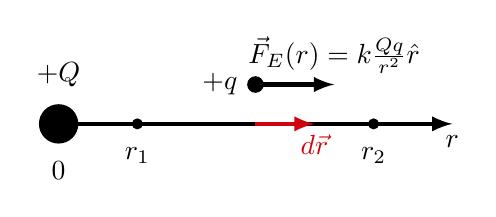
\begin{tikzpicture}
\tikzmath{
\L=5;
}
\scalebox{1}{

\coordinate (M) at (0,0);
\coordinate (mA) at (0.2*\L, 0);
\coordinate (mB) at (0.8*\L, 0);
\coordinate (mid) at ($(mA)!0.5!(mB)+(0,0.5)$);

\draw[-latex,line width=1.5] (0,0) -- (\L,0) node[below]{$r$};

\fill (M) circle (0.25) node[above=10pt]{$+Q$} node[below=10pt]{$0$};
\fill (mA) circle (2pt) node[below=5pt]{$r_1$};
\fill (mB) circle (2pt) node[below=5pt]{$r_2$};

\fill (mid) circle (3pt) node[left=3pt]{$+q$};
\draw[-latex, line width=1.5] (mid) -- +(1,0) node[above]{$\vec F_E(r)=k\frac{Qq}{r^2}\hat r$};
\draw[-latex, line width=1.5, color=myred] ($(mA)!0.5!(mB)$) -- +(0.75,0) node[below]{$d\vec r$};
}
\end{tikzpicture}
\captionof*{figure}{\textit{Determining the work done on charge $q$ in going from $\vec r_1$ to $\vec r_2$}}
\end{center}
\end{itemize}
\end{frame}




%%%%%%%%%%%%%%%%%%%%%%%%%%%%%%
\begin{frame}{Defining a function for electrical potential energy}
\vspace{-0.25cm}
\begin{center}
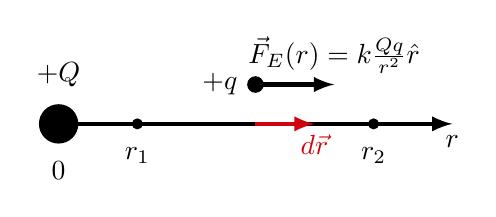
\begin{tikzpicture}
\tikzmath{
\L=5;
}
\scalebox{1}{

\coordinate (M) at (0,0);
\coordinate (mA) at (0.2*\L, 0);
\coordinate (mB) at (0.8*\L, 0);
\coordinate (mid) at ($(mA)!0.5!(mB)+(0,0.5)$);

\draw[-latex,line width=1.5] (0,0) -- (\L,0) node[below]{$r$};

\fill (M) circle (0.25) node[above=10pt]{$+Q$} node[below=10pt]{$0$};
\fill (mA) circle (2pt) node[below=5pt]{$r_1$};
\fill (mB) circle (2pt) node[below=5pt]{$r_2$};

\fill (mid) circle (3pt) node[left=3pt]{$+q$};
\draw[-latex, line width=1.5] (mid) -- +(1,0) node[above]{$\vec F_E(r)=k\frac{Qq}{r^2}\hat r$};
\draw[-latex, line width=1.5, color=myred] ($(mA)!0.5!(mB)$) -- +(0.75,0) node[below]{$d\vec r$};
}
\end{tikzpicture}
\captionof*{figure}{\textit{Determining the work done on charge $q$ in going from $\vec r_1$ to $\vec r_2$}}
\end{center}
%\capfig{0.3}{figures/potential}{Determining the work done on charge $q$ moving in a straight line.}
Calculate the work done on charge $q$ in going from $\vec r_1$ to $\vec r_2$:
\begin{align*}
W&=\int_{\vec r_1}^{\vec r_2}\vec F\cdot d\vec r = \int_{\vec r_1}^{\vec r_2}q\vec E\cdot d\vec r =kQq\int_{ r_1}^{r_2}\frac{1}{r^2}dr\\
&=kQq\left[ \frac{1}{r_1}-\frac{1}{r_2} \right] = -\Delta U = U_1 - U_2
\end{align*}
Define the potential energy function as (by inspection):
\begin{align*}
\boxed{U(r) = k\frac{Qq}{r} \textcolor{red}{+C}}
\end{align*}
\end{frame}


%%%%%%%%%%%%%%%%%%%%%%%%%%%%%%
\subsection{Choosing C}
\label{subsec:choosingC}
\begin{frame}{Choosing the constant, $C$}
\begin{align*}
U(r) = k\frac{Qq}{r} +C
\end{align*}
A simple and convenienent choice is $C=0$. This implies that the potential energy of $q$, when it is infinitely far away from $Q$, is zero. It makes sense, but is ulimately meaningless, since \textbf{only differences in potential energy are meaningful}.
\begin{align*}
\boxed{U(r) = k\frac{Qq}{r}}
\end{align*}
\end{frame}

%%%%%%%%%%%%%%%%%%%%%%%%%%%%%%


%%%%%%%%%%%%%%%%%%%%%%%%%%%%%%
\begin{frame}{What if $q$ is negative?}
Repeat the same exercise if the charge $q$ is negative:
\begin{align*}
W&=\int_{\vec r_1}^{\vec r_2}\vec F\cdot d\vec r = \int_{\vec r_1}^{\vec r_2}q\vec E\cdot d\vec r = q\int_{\vec r_1}^{\vec r_2}\vec E\cdot d\vec r =kQq\left[ \frac{1}{r_1}-\frac{1}{r_2} \right] = -\Delta U = U_1 - U_2
\end{align*}
Math is the same since $q$ factors out! That’s the whole point of defining the electric field!
\begin{align*}
\boxed{U(r) = k\frac{Qq}{r} +C}
\end{align*}
The product $qQ$ will take into account that the force changed direction (and thus the sign of the work being done depends on whether $qQ$ is positive or negative).
\end{frame}



%%%%%%%%%%%%%%%%%%%%%%%%%%%%%%
\subsection{Electric potential, $V$}
\label{subsec:electricalpotentialv}
\twocolframesf{Electric potential, $V$}
{
\begin{itemize}
\item We defined \textbf{electric field},$ \vec E$ , so that we could easily calculate the force on a charge $q$ of any sign. Electric field is \textit{force per unit charge}:
\begin{align*}
\vec F = q \vec E
\end{align*}
\item We do the same thing for potential energy! We define \textbf{electric potential}, $V$, as the \textit{potential energy per unit charge}:
\begin{align*}
U = q V
\end{align*}
\end{itemize}
}{
For a point charge, we have:
\begin{align*}
\vec F = k\frac{qQ}{r^2}\hat r \rightarrow \vec E = \frac{\vec F}{q}=k\frac{Q}{r^2}\hat r
\end{align*}
and:
\begin{align*}
U = k\frac{Qq}{r} \rightarrow V =\frac{U}{q}= k\frac{Q}{r}
\end{align*}
}

%%%%%%%%%%%%%%%%%%%%%%%%%%%%%%

%%%%%%%%%%%%%%%%%%%%%%%%%%%%%%

%%%%%%%%%%%%%%%%%%%%%%%%%%%%%%
\begin{bulletframe}{Properties of electric potential}
\item Just like potential energy, only difference in potentials are meaningful:
\begin{align*}
\Delta U &= q \Delta V\\
\Delta V &= \frac{\Delta U}{q}
\end{align*}
\item Electric potential (like potential energy) is a \textbf{scalar function of position}.
\item Potential energy relates to a specific charge, whereas potential relates to the potential energy that any charge would have.
\item \textbf{Voltage is a difference in potentials} ($\Delta V$ is a voltage). Saying that ``something is at voltage of \SI{200}{V}'' necessarily implies \textit{relative} to something else (e.g. ground). 
\end{bulletframe}

%%%%%%%%%%%%%%%%%%%%%%%%%%%%%%


%%%%%%%%%%%%%%%%%%%%%%%%




%%%%%%%%%%%%%%%%%%%%%%%%%%%%%%
\twocolframesf{Electric potential, $V$}
{
\begin{itemize}
\item We defined \textbf{electric field}, $\vec E$, so that we could easily calculate the force on a charge $q$ of any sign. Electric field is \textit{force per unit charge}:
\begin{align*}
\vec F = q \vec E
\end{align*}
\item We do the same thing for potential energy! We define \textbf{electric potential}, $V$, as \textit{potential energy per unit charge}:
\begin{align*}
U = q V
\end{align*}
\end{itemize}
}{
For a point charge, we have:
\begin{align*}
\vec F = k\frac{qQ}{r^2}\hat r \rightarrow \vec E = \frac{\vec F}{q}=k\frac{Q}{r^2}\hat r
\end{align*}
and:
\begin{align*}
U = k\frac{Qq}{r} \rightarrow V =\frac{U}{q}= k\frac{Q}{r}
\end{align*}
}

%%%%%%%%%%%%%%%%%%%%%%%%%%%%%%


%%%%%%%%%%%%%%%%%%%%%%%%%%%%%%
\twocolframesf{Electric potential}
{
\only<1,2>{
 \begin{itemize}
 \item Only differences in potential are meaningful, and they correspond to differences in potential energy
 \item All charges, if left free, will try to decrease their potential energy
 \item For a positive charge, potential energy increases with increasing potential
 \item For a negative charge, potential energy decreases with increasing potential
 \end{itemize}

 }
\only<3>{
 \capfig{0.8}{figures/Potential/honeybadger}{He really don't.}
 }
}
{
\only<1>{
\vspace{-0.5cm}
\begin{center}
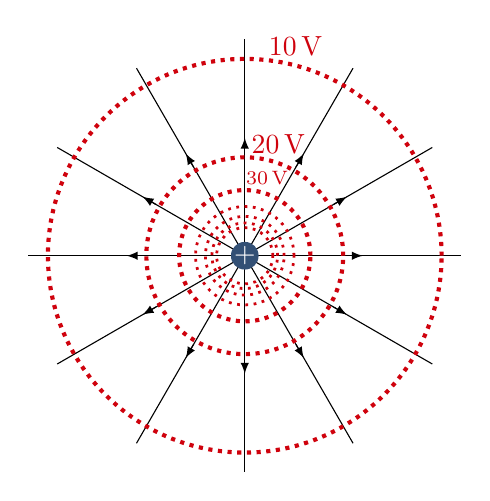
\begin{tikzpicture}
\tikzmath{
\L=2.5;
}
\scalebox{1}{

\begin{scope}
%\clip (-1.3*\L,-1.3*\L) rectangle (1.3*\L,1.3*\L);
\foreach \th in {0,30,...,330}{
\draw (0,0) -- (\th:1.1*\L);
\draw[latex-] (\th:0.6*\L) -- +(\th:-0.2);
}
\end{scope}
\fill[color=myblue!80] (0,0) circle (5pt);
\node[color=white] at (0,0){+};

\draw[dotted, color=myred, line width=1.5] (0,0) circle(\L);
\draw[dotted, color=myred, line width=1.5] (0,0) circle(\L/2);
\draw[dotted, color=myred, line width=1.5] (0,0) circle(\L/3);
\draw[dotted, color=myred, line width=1] (0,0) circle(\L/4);
\draw[dotted, color=myred, line width=1] (0,0) circle(\L/5);
\draw[dotted, color=myred, line width=1] (0,0) circle(\L/6);
\draw[dotted, color=myred, line width=1] (0,0) circle(\L/7);

\node[above,color=myred] at (75:\L){\SI{10}{V}};
\node[above,color=myred] at (70:\L/2){\SI{20}{V}};
\node[above,color=myred] at (70:\L/3){\scriptsize \SI{30}{V}};
}
\end{tikzpicture}
\captionof*{figure}{\textit{Point charge: electric field and potential.}}
\end{center}
%\capfig{0.8}{figures/fig2}{Point charge: electric field and potential}
}
\only<2->{
\begin{center}
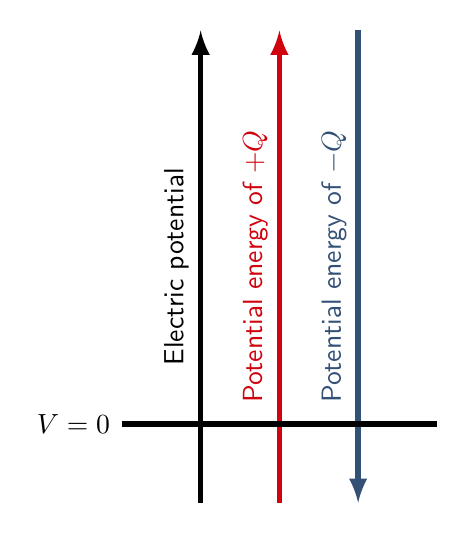
\begin{tikzpicture}
\tikzmath{
\h=6;
}
\scalebox{1}{
\draw[-latex,line width=2] (0,0) -- +(0,\h)node[midway, above,rotate=90]{Electric potential};
\draw[-latex,line width=2,color=myred] (1,0) -- +(0,\h)node[midway, above,rotate=90]{Potential energy of $+Q$};
\draw[latex-,line width=2,color=myblue!80] (2,0) -- +(0,\h)node[midway, above,rotate=90]{Potential energy of $-Q$};
\only<3>{
\draw[line width=2] (-1,1) node[left]{$V=0$} -- (3,1);
}
}
\end{tikzpicture}
\captionof*{figure}{\textit{Potential and potential energy.}}
\end{center}
}
}



%%%%%%%%%%%%%%%%%%%%%%%%%%%%%%
\twocolframe{Potential and Potential Energy}
{
\vspace{-0.25cm}
\textbf{Gravitational Force}
{\footnotesize 
\begin{itemize}
\item Force:
\begin{align*}
\vec F = \frac{GMm}{r^2}\hat r
\end{align*}

\item Field (force per unit mass) near \textbf{point mass $M$}:
\begin{align*}
\vec g = \frac{GM}{r^2}\hat r
\end{align*}

\item Potential energy near \textbf{point mass $M$}:
\begin{align*}
U(r) = -\frac{GMm}{r}+C=-\int \vec F\cdot d \vec r
\end{align*}

\item ``Potential'' \textbf{from point mass $M$} (potential energy per unit mass):
\begin{align*}
V(r) = -\frac{GM}{r}+C=-\int \vec g\cdot d \vec r
\end{align*}
\end{itemize}
}
}
{
\vspace{-0.25cm}
\textbf{Electric Force}
{\footnotesize 

\begin{itemize}
\item Force:
\begin{align*}
\vec F = \frac{kQq}{r^2}\hat r
\end{align*}

\item Field (force per unit \textit{charge}) near \textbf{point \textit{charge} $Q$}:
\begin{align*}
\vec E = \frac{kQ}{r^2}\hat r
\end{align*}

\item Potential energy near \textbf{point \textit{charge} $Q$}:
\begin{align*}
U(r) = -\frac{kQq}{r}+C=-\int \vec F\cdot d \vec r
\end{align*}

\item ``Potential'' \textbf{from point \textit{charge} $Q$} (potential energy per unit \textit{charge}):
\begin{align*}
V(r) = -\frac{kQ}{r}+C=-\int \vec E\cdot d \vec r
\end{align*}
\end{itemize}
}
}

%%%%%%%%%%%%%%%%%%%%%%%




%%%%%%%%%%%%%%%%%%%%%%%%%%%%%%%%
\section{Calculating Electric Potential}
\label{sec:calculatingelectricpotential}
\title{Calculating Electric Potential}


%%%%%%%%%%%%%%%%%%%%%%%%%
\begin{frame}
\titlepage
\thispagestyle{empty}
\end{frame}

%%%%%%%%%%%%%%%






%%%%%%%%%%%%%%%%%%%%%%%%%%%%%%
\begin{frame}{Calculating electric potential}
Work done by the force gives potential energy:
\begin{align*}
W&=\int_{\vec r_1}^{\vec r_2}\vec F\cdot d\vec r = \int_{\vec r_1}^{\vec r_2}q\vec E\cdot d\vec r = \textcolor{red}{q}\int_{\vec r_1}^{\vec r_2}\vec E\cdot d\vec r = -\Delta U 
\end{align*}
Doing this per charge, gives electric potential
\begin{align*}
-\Delta V = \frac{-\Delta U}{q}=\int_{\vec r_1}^{\vec r_2}\vec E\cdot d\vec r 
\end{align*}
Electric potential is to electrical potential energy what electric field is to electric force:
\begin{align*}
\Delta U &= -\int_{\vec r_1}^{\vec r_2} \textcolor{red}{\vec F}\cdot d\vec r\\
\Delta V &= -\int_{\vec r_1}^{\vec r_2} \textcolor{red}{\vec E}\cdot d\vec r
\end{align*}
\end{frame}

%%%%%%%%%%%%%%%%%%%%%%%%%%%%%%

%%%%%%%%%%%%%%%%%%%%%%%%%%%%%
\subsection{Methods of determining electric potential}
\label{subsec:methodsofdeterminingelectricpotential}
\twocolframest{Two methods to determine electric potential}
{
\begin{enumerate}
\item \textbf{Use the electric field} and integrate it (if you already know the electric field):
\begin{align*}
\Delta V &= (V_2-V_1) = -\int_{\vec r_1}^{\vec r_2} \vec E\cdot d\vec r\\
V(\vec r)&= -\int \vec E \cdot d\vec r
\end{align*}
\item \textbf{Model as a collection of point charges} and sum the potentials (\textcolor{myred}{Make sure they share the location of \SI{0}{V}!}):
\begin{align*}
dV&=\frac{kdq}{r}\\
\therefore V &= \int dV = k \int \frac{dq}{r}
\end{align*}
\end{enumerate}
}
{
\begin{block}{Using the $E$-field}
This is what we did to determine the potential near a point charge $Q$
\end{block}
\vspace{2cm}
\begin{block}{Summing the potentials}
This is analogous to how we calculate the electric field for a distributed charge, but much easier since potential is a scalar!
\end{block}
}

%%%%%%%%%%%%%%%%%%%%%%%%%%%%%%



\subsection{Electric potential near a point charge}
\label{subsec:electricpotentialnearapointcharge}
\begin{frame}{Electric potential near a point charge, $Q$}

\begin{itemize}
\item We can calculate the potential energy function from the anti-derivative:
\begin{align*}
V(r) &= -\int \textcolor{red}{\vec E}\cdot d\vec r = -\int k\frac{Q}{r^2}dr = k\frac{Q}{r}+C\\
\end{align*}
\item \textbf{If we define zero potential energy at infinity ($C = 0$)}, then this also corresponds to zero electric potential, and we can define electric potential from a point charge as:
\begin{align*}
 V(r) =k\frac{Q}{r}
\end{align*}
\end{itemize}
\end{frame}
%%%%%%%%%%%%%%%%%%%%%%%%%%%%%%%%
\twocolframest{Electric potential energy near point charge, $Q$}
{
\begin{itemize}
\item Found the potential energy of q a distance r from Q:\\
\begin{align*}
U(r) = \frac{kQq}{r}+C
\end{align*}
\item Convenient choice is $C=0$
\item This means that we explicitly define $U(r)=0$ when $r\to\infty$:
\begin{align*}
\boxed{U(r) = \frac{kQq}{r}}
\end{align*}

\end{itemize}
}
{
\begin{center}
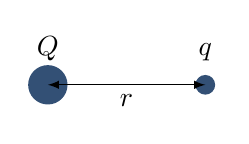
\begin{tikzpicture}
\tikzmath{
\L=2;
\R=0.25;
}
\scalebox{1}{

\fill[color=myblue!80] (0,0) circle(\R) node[above=5pt,color=black]{$Q$};
\fill[color=myblue!80] (\L,0) circle(\R/2) node[above=5pt,color=black]{$q$};
\draw[latex-latex] (0,0) -- (\L,0) node[midway,below]{$r$};
}
\end{tikzpicture}
\captionof*{figure}{\textit{Point charges separated by distance, $r$.}}
\end{center}
}



%%%%%%%%%%%%%%%%%%%%%%%%%%%%%%
\subsection{Potential from a ring of charge}
\label{subsec:potentialfromaringofcharge}
\twocolframesf{Potential from a ring of charge, along symmetry axis}
{
\begin{itemize}
\item Break it up into many small point charges, $dq$.
\item Write the potential from a $dq$:
\begin{align*}
dV&=\frac{kdq}{r}=\frac{kdq}{\sqrt{R^2+x^2}}
\end{align*}
\item Sum the potentials (integrate):
\begin{align*}
\therefore V &= \int dV = \int_0^Q \frac{kdq}{\sqrt{R^2+x^2}} = \frac{kQ}{\sqrt{R^2+x^2}}
\end{align*}
\end{itemize}
\only<1>{
\begin{alertblock}{Careful!}
This only works if all the potentials, $dV$, have the same locations defined for \SI{0}{V} (namely, at infinity, since we chose $C=0$).
\end{alertblock}
}
\only<2>{
\begin{block}{Easy integrand!}
We don't need to express $dq$ with a position variable (e.g. $dq=\lambda R d\theta$) since all quantities in the integrand are constants! But you should try to convince yourself you'll get the same answer!
\end{block}
}
}
{
%\capfig{0.5}{figures/potential_ring}{A point charge, $dq$, on the ring}
\begin{center}
\begin{tikzpicture}
\tikzmath{
\L=2.5;
\R=0.5*\L;
\thperp=45;
\Px=0.5*\L;
\dtheta=20;
}
\scalebox{1}{

\draw[-latex] (0,0) -- +(\L,0) node[below]{$x$};
\draw[-latex] (0,0) -- +(0,\L) node[left]{$z$};
\draw[-latex,dashed] (0,0) -- +(\thperp:0.75*\L) node[right]{$y$};

\draw[line width=1.5] (0,\R) arc(90:270:{\R/4} and {\R});
\draw[line width=1] (0,\R) arc(90:-90:{\R/4} and {\R});

\node[above left] at (0,\R) {$Q$};
\node[above, color=myred] at (0.5*\Px,0) {$x$};
\fill (\Px,0) circle (2pt) node[above]{$P$};
\draw[color=myred, line width=1.5] (270+\dtheta:{\R/4} and {\R}) arc (270+\dtheta:270-\dtheta:{\R/4} and {\R}) node[midway,below]{$dq$};

\draw[color=myred, line width=1.5, dotted] (270:{\R/4} and {\R}) -- (\Px,0) node[midway,right]{$\sqrt{R^2+r^2}$};
\only<1>{
\draw[dotted, line width=1] (0,0) -- (225:{\R/4} and {\R}) node[midway,right=-2pt]{$R$};
}
\only<2>{

\draw[color=myred] (0,0) -- (270+\dtheta:{\R/4} and {\R}) ;
\draw[color=myred] (0,0) -- (270-\dtheta:{\R/4} and {\R}) ;
\draw[-latex, color=myred] (-\R/2,-\R/2) node[left]{$d\theta$} -- (0,-\R/2);
}
}
\end{tikzpicture}
\captionof*{figure}{\textit{A point charge, $dq$, on a ring of radius, $R$.}}
\end{center}

}


%%%%%%%%%%%%%%%%%%%%%%%%%%%%%%
\twocolframesf{Potential from a disk carrying surface charge, $\sigma$}
{
\begin{itemize}
\item Break up the disk into \textcolor{red}{small rings} of charge, $\textcolor{red}{dq}$, and radius, $\textcolor{red}{r}$. Each ring has an area $dA$:
\begin{align*}
dq = \sigma dA = \sigma 2\pi r dr
\end{align*}
\item Write the potential from $dq$ (using our previous result):
\begin{align*}
dV = \frac{kdq}{\sqrt{r^2+x^2}}=\frac{k\sigma 2\pi r dr}{\sqrt{r^2+x^2}}
\end{align*}
\item Sum the potentials:
\begin{align*}
\therefore V = \int dV = 2\pi k \sigma \int_0^R \frac{ r}{\sqrt{r^2+x^2}}dr
\end{align*}
\end{itemize}
}
{

\begin{center}
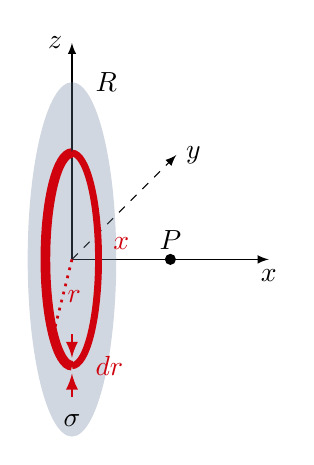
\begin{tikzpicture}
\tikzmath{
\L=2.5;
\R=0.9*\L;
\Rdq=0.6*\R;
\thperp=45;
\Px=0.5*\L;
\dtheta=20;
}
\scalebox{1}{

\draw[-latex] (0,0) -- +(\L,0) node[below]{$x$};
\draw[-latex] (0,0) -- +(0,1.1*\L) node[left]{$z$};
\draw[-latex,dashed] (0,0) -- +(\thperp:0.75*\L) node[right]{$y$};

\fill[color=myblue!60,opacity=0.3] (0,0) circle ({\R/4} and {\R});

\draw[line width=3.5,color=myred] (0,\Rdq) arc(90:270:{\Rdq/4} and {\Rdq});
\draw[line width=2.5,color=myred] (0,\Rdq) arc(90:-90:{\Rdq/4} and {\Rdq});


\fill (\Px,0) circle (2pt) node[above]{$P$};
\node[above, color=myred] at (0.5*\Px,0) {$x$};

\draw[dotted, line width=1, color=myred] (0,0) -- (225:{\Rdq/4} and {\Rdq}) node[midway,right=-2pt]{$r$};

\draw[color=myred,line width=1, latex-] (0,-\Rdq+0.1) -- +(0,0.3);
\draw[color=myred,line width=1, latex-] (0,-\Rdq-0.1) -- +(0,-0.3);
\node[color=myred, right=5pt] at (0,-\Rdq){$dr$};
\node[right=5pt] at (0,\R) {$R$};
\node[above] at (0,-\R) {$\sigma$};
}
\end{tikzpicture}
\captionof*{figure}{\textit{A ring of charge $dq$ on a disk carrying surface charge $\sigma$. Think of unfolding the ring into a rectangle of length $2\pi r$ and height $dr$ to determine its area, $dA$.}}
\end{center}

}


%%%%%%%%%%%%%%%%%%%%%%%%%%%%%%



%%%%%%%%%%%%%%%%%%%%%%%%%%%%%%
\subsection{Getting $\vec E$ from $V$}
\label{subsec:gettingefromv}
\twocolframesf{What about $\vec E$ from $V$?}
{
\begin{itemize}
\item If we know the electric field vector, by using a scalar product ($q\vec E \cdot d\vec r$), we can find the electric potential (vector $\to$ scalar)
\item How do we go the other way (scalar $\to$ vector)?
\begin{itemize}
\item Based on the direction in which electric potential increases, we can \textbf{determine the direction of the field}.
\item Based on how quickly the potential changes, we can determine the \textbf{magnitude of the field}. 
\end{itemize}

\end{itemize}
}
{
\capfig{1}{figures/Potential/contours}{Contour lines on a map}
\begin{block}{Contour lines}
Lines (contours) of constant electric potential correspond to lines of constant electric potential energy. Just like lines of constant altitude correspond to lines of constant gravitational potential energy.
\end{block}
}



%%%%%%%%%%%%%%%%%%%%%%%%%%%%%%
\twocolframesf{$\vec E$ from $V$ in 1D}
{
\begin{itemize}
\item $V$ from $\vec E$:
\begin{align*}
V(x) = -\int E dx
\end{align*}
\item $\vec E$ from $V$
\begin{align*}
\therefore E(x) = -\frac{dV}{dx}=-k
\end{align*}
\item Electric potential is the (negative) anti-derivative of electric field (in 1D).
\item Electric field  is this the (negative) derivative of electric potential.
\end{itemize}

}
{
%\capfig{0.35}{figures/potential_linear}{Example of a linear potential}
\begin{center}
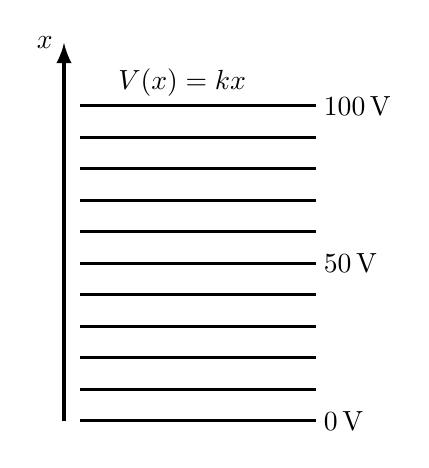
\begin{tikzpicture}
\tikzmath{
\h=4;
\L=3;
}
\scalebox{1}{

\draw[-latex, line width =1.5] (0,0) -- +(0,1.2*\h) node[left]{$x$};

\foreach \i in {0,0.1,...,1.1}{
 \draw[line width =1] (0.2,\i*\h) -- +(\L,0);
}

\node[above] at (\L/2,\h){$V(x)=kx$};
\node[right=5pt] at (\L,0){\SI{0}{V}};
\node[right=5pt] at (\L,0.5*\h){\SI{50}{V}};
\node[right=5pt] at (\L,\h){\SI{100}{V}};
}
\end{tikzpicture}
\captionof*{figure}{\textit{Example of a linear potential.}}
\end{center}
}


%%%%%%%%%%%%%%%%%%%%%%%%%%%%%%
\twocolframest{$\vec E$ from $V$ in 3D}
{
\vspace{-0.5cm}
\begin{itemize}
\item $V$ from $\vec E$:
\begin{align*}
V(\vec r)= V(x,y,z) = -\int \vec E \cdot  d\vec r
\end{align*}
\item $\vec E$ from $V$
\begin{align*}
E_x &= -\frac{\partial V}{\partial x}\\
E_y &= -\frac{\partial V}{\partial y}\\
E_z &= -\frac{\partial V}{\partial z}
\end{align*}
\item In 3D, we need to know how the potential changes (its derivatives) in each direction. Those (partial) derivatives are the 3 components of the electric field!
\end{itemize}

}
{
\begin{block}{Different Notation}
The electric field is the (negative) gradient of the electric potential:
\begin{align*}
\vec E &= -\nabla V\\
&=-\left( \frac{\partial V}{\partial x} \hat x + \frac{\partial V}{\partial y}\hat y+\frac{\partial V}{\partial z}\hat z\right)
\end{align*}
\end{block}
}


%%%%%%%%%%%%%%%%%%%%%%%%%%%%%%





%%%%%%%%%%%%%%%%%%%%%%%%%%%%%%%%
\section{Application}
\label{sec:application}
\title{Application}


%%%%%%%%%%%%%%%%%%%%%%%%%
\begin{frame}
\titlepage
\thispagestyle{empty}
\end{frame}

%%%%%%%%%%%%%%%



%%%%%%%%%%%%%%%%%%%%%%%%
\subsection{Gradient vector review}
\label{subsec:gradientvectorreview}
\twocolframe{Recall the gradient vector}
{
\begin{itemize}
\item From the partial derivatives, we know how the function changes along the $x$ and $y$ directions
\item The gradient tells us the direction in which the function changes the fastest (in which direction the slope is the steepest)
\item It is a vector whose magnitude tells us how fast the function is changing in the direction of maximal change.
\begin{align*}
\nabla f(x,y) &= \frac{\partial f}{\partial x} \hat x + \frac{\partial f}{\partial y}\hat y\\
&=2x\hat x - 4y \hat y = (-4,8)
\end{align*}
\end{itemize}
}
{
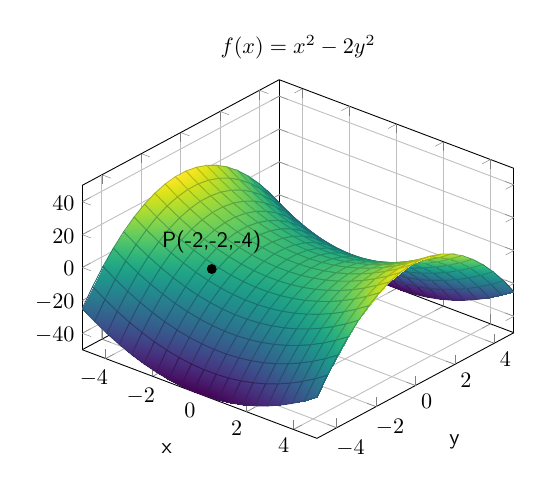
\begin{tikzpicture}[scale=0.8]

\begin{axis}[
  colormap/viridis,  
  view = {40}{40},
	xmax = 5,
	xmin = -5,
	ymax = 5, 
	ymin = -5, 
	zmax = 50, 
	zmin = -50,
	xtick = {-4,-2,0,2,4},
	ytick = {-4,-2,0,2,4},
	ztick = {-40,-20,0,20,40},
	xlabel={x},
	ylabel={y},
	title={$f(x)=x^2-2y^2$},
	grid]
	

\addplot3 [
	domain=-5:5,
	domain y = -5:5,
	samples = 20,
	samples y = 20,
	surf,
	shader =faceted interp] {x^2 -2*y^2};
	
\node[label={P(-2,-2,-4)}] at (-2,-2,-4) {};
\draw plot [mark=*, mark size=2] coordinates{(-2,-2,-4)}; 

\end{axis}

\end{tikzpicture}
\captionof*{figure}{\textit{A point, $P$, is on the surface given by $f(x,y)=x^2-2y^2$.}}
}


%%%%%%%%%%%%%%%%%%%%%%%%%%%%%%
\twocolframe{Recall the gradient vector}
{
\begin{itemize}
\item From the partial derivatives, we know how the function changes along the $x$ and $y$ directions
\item The gradient tells us the direction in which the function changes the fastest (in which direction the slope is the steepest)
\item It is a vector whose magnitude tells us how fast the function is changing in the direction of maximal change.
\begin{align*}
\nabla f(x,y) &= \frac{\partial f}{\partial x} \hat x + \frac{\partial f}{\partial y}\hat y\\
&=2x\hat x - 4y \hat y = (-4,8)
\end{align*}
\end{itemize}
}
{
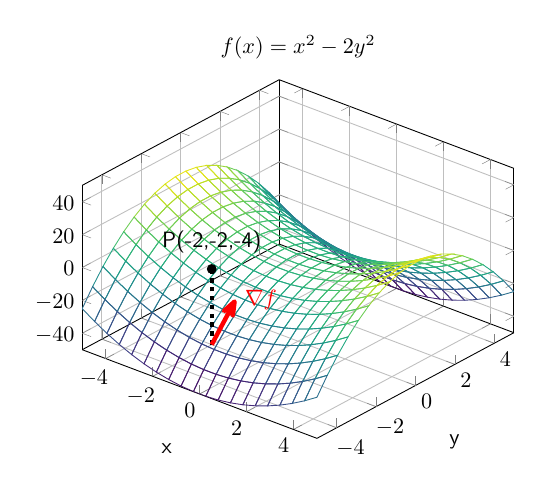
\begin{tikzpicture}[scale=0.8]
\usetikzlibrary {arrows.meta} 
\begin{axis}[
  colormap/viridis,  
  view = {40}{40},
	xmax = 5,
	xmin = -5,
	ymax = 5, 
	ymin = -5, 
	zmax = 50, 
	zmin = -50,
	xtick = {-4,-2,0,2,4},
	ytick = {-4,-2,0,2,4},
	ztick = {-40,-20,0,20,40},
	xlabel={x},
	ylabel={y},
	title={$f(x)=x^2-2y^2$},
	grid]
	

\addplot3 [
	domain=-5:5,
	domain y = -5:5,
	samples = 20,
	samples y = 20,
	mesh,
	%fill opacity=0.5,
	shader =faceted interp] {x^2 -2*y^2};
	
\draw[line width=2pt,dotted] (-2,-2,-50) -- (-2,-2,-4)	;
\node[label={P(-2,-2,-4)}] at (-2,-2,-4) {};
\draw plot [mark=*, mark size=2] coordinates{(-2,-2,-4)}; 
\draw[line width=2pt,red,-{Stealth[round]}] (-2,-2,-50)--(-3.5,1,-50) node[right]{$\nabla f$};

\end{axis}

\end{tikzpicture}
\captionof*{figure}{\textit{A vector parallel to the gradient vector is projected in the $xy$-plane. It points in the direction of most rapid increase.}}
}


\begin{bulletframe}{Gradient in physics}
\item The \textbf{gradient of the potential energy} tells us in which direction the \textbf{corresponding force} is exerted. The force is exerted in the opposite direction of the gradient vector (the force is exerted in the direction opposite to that which potential energy increases).
\begin{itemize}
\item Think of a contour map in the context of gravity. The contours are regions of constant elevation (namely, constant gravitational potential energy).
\end{itemize}
\item The \textbf{gradient of the electric potential} tells us in which direction the \textbf{corresponding electric field} is. The field is in the opposite direction of  the gradient vector.
\end{bulletframe}

%%%%%%%%%%%%%%%%%%%%%%%%%%




%%%%%%%%%%%%%%%%%%%%%%%%%%%%%%%%
\subsection{Electric potential summary}
\label{subsec:electricpotentialsummary}
\begin{bulletframe}{Summary: Electric Potential}
 \item We started with Coulomb’s Law for the \textbf{electric force vector} between 2 points charges: $\vec F$
 \item We defined the \textbf{electric field vector}, which is independent of the ``test'' charge, $q$: $\vec F=q\vec E$
 \item Knowing that the force is conservative, we defined a (scalar) \textbf{potential energy function}: $U(\vec r)$
 \item We defined the \textbf{electric potential function}, which is independent of the test charge, $q$: $U(\vec r) = q V(\vec r)$
 \item[$\rightarrow$] We can now describe the motion of electric charges using scalar quantities (electric potential and electric potential energy).
 \item[$\rightarrow$] Instead of an electric force vector acting in certain direction, you can think of charges moving to regions of space where they will lower the electric potential energy.
\end{bulletframe}



%%%%%%%%%%%%%%%%%%%%%%%%%%%%%%


%%%%%%%%%%%%%%%%%%%%%%%%%%%%%%
\subsection{Equipotential surfaces}
\label{subsec:equipotentialsurfaces}
\twocolframesf{Equipotential surfaces}
{
\begin{itemize}
  \item Electric potential is a scalar function of position, $V(x,y,z)$.
  \item Electric potential gives the electric potential energy of a charge at a given position.
  \item \textbf{Equipotential surfaces} are regions of space where electric potential is constant.
  \item The electric field does not do work along an equipotential surface.
  \item Conductors are always equipotentials (the net field inside a conductor must be zero in electrostatics, so the potential cannot change inside a conductor). 
\end{itemize}
}
{
\begin{center}
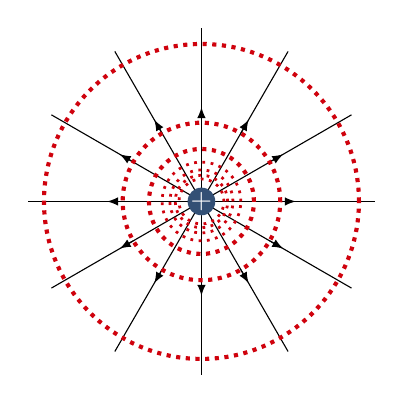
\begin{tikzpicture}
\tikzmath{
\L=2;
}
\scalebox{1}{

\begin{scope}
%\clip (-1.3*\L,-1.3*\L) rectangle (1.3*\L,1.3*\L);
\foreach \th in {0,30,...,330}{
\draw (0,0) -- (\th:1.1*\L);
\draw[latex-] (\th:0.6*\L) -- +(\th:-0.2);
}
\end{scope}
\fill[color=myblue!80] (0,0) circle (5pt);
\node[color=white] at (0,0){+};

\draw[dotted, color=myred, line width=1.5] (0,0) circle(\L);
\draw[dotted, color=myred, line width=1.5] (0,0) circle(\L/2);
\draw[dotted, color=myred, line width=1.5] (0,0) circle(\L/3);
\draw[dotted, color=myred, line width=1] (0,0) circle(\L/4);
\draw[dotted, color=myred, line width=1] (0,0) circle(\L/5);
\draw[dotted, color=myred, line width=1] (0,0) circle(\L/6);
\draw[dotted, color=myred, line width=1] (0,0) circle(\L/7);

}
\end{tikzpicture}
\captionof*{figure}{\textit{For a point charge, equipotential surfaces consist in concentric spheres; the electric field foes no work along one of these surfaces.}}
\end{center}



}




%%%%%%%%%%%%%%%%%%%%%%%%%%%%%%
\twocolframesf{Equipotential surfaces}
{
\begin{itemize}
  \item Since they are regions of constant electric potential energy, the electric field does no work when moving along an equipotential
  \item The equipotential surfaces are always perpendicular to the electric field lines:
  \begin{align*}
  W = \vec F \cdot \vec d = Fd\cos\theta
  \end{align*}
  \item[$\rightarrow$]  Electric field is always perpendicular to surface of the conductor

\end{itemize}
}
{
\begin{center}
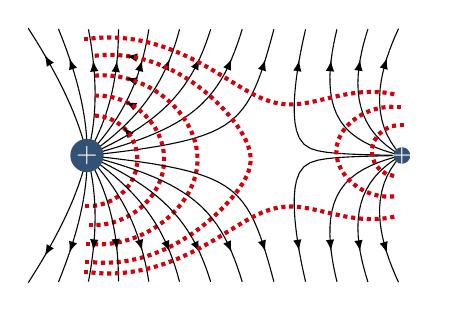
\begin{tikzpicture}
\tikzmath{
\xe=-2;%Coordinates of first mass/charge (Earth)
\ye=0;
\xm=2;%Coordinates of first mass/charge (Moon)
\ym=0;
\mee=1;% Mass/charge of first mass (Earth)
\mmm=0.6;% Mass/charge of first mass (Earth)
\dl=0.1;%scale factor to advance along the field line
\n=35;%number of points to find in the line (make as small as possible to reach the point you want!)
\nequi=60;
}

\scalebox{1}{
%Top field lines (xst is the starting x position of the field line)
\foreach \xst in {-2.8,-2.4,...,2.4}{
  \tikzmath{
  \yst=1.7; %all field lines start at yst
  \x=\xst;
  \y=\yst;
  %
  %generate points on the line (keeps finding the next point)
  int \i;
  %note that this also creates \mypairx and \mypairy!
  coordinate \mypair;
  for \i in {1,...,\n}{
    %First mass (earth)
    \re=(\x-\xe)*(\x-\xe)+(\y-\ye)*(\y-\ye)+0.0001;
    \Fex=\mee*(\x-\xe)/\re;
    \Fey=\mee*(\y-\ye)/\re;
    %Second mass (moon)
    \rm=(\x-\xm)*(\x-\xm)+(\y-\ym)*(\y-\ym)+0.0001;
    \Fmx=\mmm*(\x-\xm)/\rm;
    \Fmy=\mmm*(\y-\ym)/\rm;
    %Total force:
    \Fx=\Fex+\Fmx;
    \Fy=\Fey+\Fmy;
    \Fn=sqrt(\Fx*\Fx+\Fy*\Fy)+0.0001;
    \dx=\Fx/\Fn*\dl;
    \dy=\Fy/\Fn*\dl; 
    \x=\x-\dx;
    \y=\y-\dy;
    \mypair{\i}=(\x,\y);
    };
  }
  %Draw that field line
  \foreach \i in {2,...,\n}{
    \tikzmath{
    int \im;
    \im=\i-1;
    }
    \draw (\mypair{\im}) -- (\mypair{\i});
    \ifthenelse{\im =5}{\draw[latex-] (\mypair{\im}) -- (\mypair{\i})}{};%draw arrow on the fifth point
  }

}%end of loop over x

%equipotential:
\foreach \yst in {0.5,0.75,1, 1.25}{
  \tikzmath{
  \xst=\xe;
  %\yst=0.75; %all field lines start at yst
  \x=\xst;
  \y=\yst;
  %
  %generate points on the line (keeps finding the next point)
  int \i;
  %note that this also creates \mypairx and \mypairy!
  coordinate \mypair;
  for \i in {1,...,\nequi}{
    %First mass (earth)
    \re=(\x-\xe)*(\x-\xe)+(\y-\ye)*(\y-\ye)+0.0001;
    \Fex=\mee*(\x-\xe)/\re;
    \Fey=\mee*(\y-\ye)/\re;
    %Second mass (moon)
    \rm=(\x-\xm)*(\x-\xm)+(\y-\ym)*(\y-\ym)+0.0001;
    \Fmx=\mmm*(\x-\xm)/\rm;
    \Fmy=\mmm*(\y-\ym)/\rm;
    %Total force:
    \Fx=\Fex+\Fmx;
    \Fy=\Fey+\Fmy;
    \Fn=sqrt(\Fx*\Fx+\Fy*\Fy)+0.0001;
    \dx=-\Fy/\Fn*\dl;
    \dy=\Fx/\Fn*\dl;
    \x=ifthenelse(\x>-2.001,\x-\dx,\x);
    \y=ifthenelse(\x>-2.001,\y-\dy,\y);
    \mypair{\i}=(\x,\y);
    };
  }
  %Draw that field line
  \foreach \i in {2,...,\nequi}{
    \tikzmath{
    int \im;
    \im=\i-1;
    }
    \draw[color=myred,dotted,line width=1.5] (\mypair{\im}) -- (\mypair{\i});
    //\ifthenelse{\im =5}{\draw[latex-] (\mypair{\im}) -- (\mypair{\i})}{};%draw arrow on the fifth point
  }

}%end of loop over x

%Bottom field lines
\foreach \xst in {-2.8,-2.4,...,2.4}{
  \tikzmath{
  \yst=-1.7;
  \x=\xst;
  \y=\yst;
  %
  %generate points on the line
  int \i;
  %note that this also creates \mypairx and \mypairy!
  coordinate \mypair;
  for \i in {1,...,\n}{
    %First mass (earth)
    \re=(\x-\xe)*(\x-\xe)+(\y-\ye)*(\y-\ye)+0.0001;
    \Fex=\mee*(\x-\xe)/\re;
    \Fey=\mee*(\y-\ye)/\re;
    %Second mass (moon)
    \rm=(\x-\xm)*(\x-\xm)+(\y-\ym)*(\y-\ym)+0.0001;
    \Fmx=\mmm*(\x-\xm)/\rm;
    \Fmy=\mmm*(\y-\ym)/\rm;
    %Total force:
    \Fx=\Fex+\Fmx;
    \Fy=\Fey+\Fmy;
    \Fn=sqrt(\Fx*\Fx+\Fy*\Fy)+0.0001;
    \dx=\Fx/\Fn*\dl;
    \dy=\Fy/\Fn*\dl;
    \x=\x-\dx;
    \y=\y-\dy;
    \mypair{\i}=(\x,\y);
     };
  }
  %Draw that field line
  \foreach \i in {2,...,\n}{
    \tikzmath{
      int \im;
      \im=\i-1;
    }
    \draw (\mypair{\im}) -- (\mypair{\i});
    \ifthenelse{\im =5}{\draw[latex-] (\mypair{\im}) -- (\mypair{\i})}{};
  }

}%end of loop over x


%equipotential:
\foreach \yst in {-0.25, -0.5,-0.75}{
  \tikzmath{
  \xst=\xm;
  %\yst=0.75; %all field lines start at yst
  \x=\xst;
  \y=\yst;
  %
  %generate points on the line (keeps finding the next point)
  int \i;
  %note that this also creates \mypairx and \mypairy!
  coordinate \mypair;
  for \i in {1,...,\nequi}{
    %First mass (earth)
    \re=(\x-\xe)*(\x-\xe)+(\y-\ye)*(\y-\ye)+0.0001;
    \Fex=\mee*(\x-\xe)/\re;
    \Fey=\mee*(\y-\ye)/\re;
    %Second mass (moon)
    \rm=(\x-\xm)*(\x-\xm)+(\y-\ym)*(\y-\ym)+0.0001;
    \Fmx=\mmm*(\x-\xm)/\rm;
    \Fmy=\mmm*(\y-\ym)/\rm;
    %Total force:
    \Fx=\Fex+\Fmx;
    \Fy=\Fey+\Fmy;
    \Fn=sqrt(\Fx*\Fx+\Fy*\Fy)+0.0001;
    \dx=-\Fy/\Fn*\dl;
    \dy=\Fx/\Fn*\dl;
    \x=ifthenelse((\x<2.001) && (\x>-2.001),\x-\dx,\x);
    \y=ifthenelse((\x<2.001) && (\x>-2.001),\y-\dy,\y);
    \mypair{\i}=(\x,\y);
    };
  }
  %Draw that field line
  \foreach \i in {2,...,\nequi}{
    \tikzmath{
    int \im;
    \im=\i-1;
    }
    \draw[color=myred,dotted,line width=1.5] (\mypair{\im}) -- (\mypair{\i});
  }

}%end of loop over x


%equipotential:
\foreach \yst in {0.75}{
  \tikzmath{
  \xst=\xm;
  %\yst=0.75; %all field lines start at yst
  \x=\xst;
  \y=\yst;
  %
  %generate points on the line (keeps finding the next point)
  int \i;
  %note that this also creates \mypairx and \mypairy!
  coordinate \mypair;
  for \i in {1,...,\nequi}{
    %First mass (earth)
    \re=(\x-\xe)*(\x-\xe)+(\y-\ye)*(\y-\ye)+0.0001;
    \Fex=\mee*(\x-\xe)/\re;
    \Fey=\mee*(\y-\ye)/\re;
    %Second mass (moon)
    \rm=(\x-\xm)*(\x-\xm)+(\y-\ym)*(\y-\ym)+0.0001;
    \Fmx=\mmm*(\x-\xm)/\rm;
    \Fmy=\mmm*(\y-\ym)/\rm;
    %Total force:
    \Fx=\Fex+\Fmx;
    \Fy=\Fey+\Fmy;
    \Fn=sqrt(\Fx*\Fx+\Fy*\Fy)+0.0001;
    \dx=-\Fy/\Fn*\dl;
    \dy=\Fx/\Fn*\dl;
    \x=ifthenelse((\x<2.001) && (\x>-2.001),\x+\dx,\x);
    \y=ifthenelse((\x<2.001) && (\x>-2.001),\y+\dy,\y);
    \mypair{\i}=(\x,\y);
    };
  }
  %Draw that field line
  \foreach \i in {2,...,\nequi}{
    \tikzmath{
    int \im;
    \im=\i-1;
    }
    \draw[color=myred,dotted,line width=1.5] (\mypair{\im}) -- (\mypair{\i});
  }

}%end of loop over x

%Draw the charges
\fill[color=myblue!80] ((\xe,\ye)  circle (6pt);
\node[color=white] at (\xe,\ye) {$+$};

\fill[color=myblue!80] (\xm,\ym) circle (3pt);
\node[color=white] at (\xm,\ym){$+$};


}

\end{tikzpicture}
\captionof*{figure}{\textit{Electric field lines and corresponding equipotentials from two unequal positive charges.}}
\end{center}
}


%%%%%%%%%%%%%%%%%%%%%%%%%%%%%%





%%%%%%%%%%%%%%%%%%%%%%%%%%%%%%
\subsection{Charges on the surface of a conductor}
\label{subsec:chargesonthesurfaceofaconductor}
\twocolframesf{Charges on the surface of a conductor}
{
\begin{itemize}
  \item Charges spread uniformly on the outer \textbf{surface} of a conducting sphere.
  \item Gauss' Law:
  \begin{align*}
  (4\pi r^2) E(r) = \frac{Q}{\epsilon_0}\rightarrow E(r) = \frac{1}{4\pi \epsilon_0}\frac{Q}{r^2}
  \end{align*}
  \item At some distance, $r$, the potential is given by:
  \begin{align*}
    V(r) = \frac{1}{4\pi \epsilon_0}\frac{Q}{r}\quad\left(V(r\to\infty)=0\right)
  \end{align*}
  \item[$\rightarrow$] For a charged sphere, evaluating $V$ and $E$ at $r=R$, we thus have:
  \begin{align*}
    \boxed {V=ER}
  \end{align*}
\end{itemize}
}
{
\vspace{-1cm}
\begin{center}

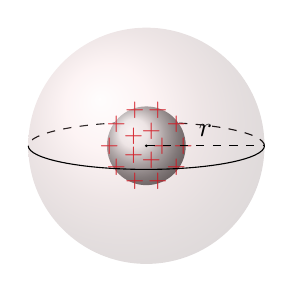
\begin{tikzpicture}[scale=0.5]
  \tikzmath{
    \Rout=1;
  }
  
  \draw[dashed] (3,0) arc (0:180:3 and 0.6);
  \shade[ball color = gray!20, opacity = 1] (0,0) circle (1cm);
  
  \foreach \i [evaluate={\ang=0+\i*360/10;}] in {1,...,10}{
    \node[myred,scale=0.9] at (\ang:0.94*\Rout) {\textbf{$+$}};
  }
  \foreach \i [evaluate={\ang=0+\i*360/5;}] in {1,...,5}{
    \node[myred,scale=0.9] at (\ang:0.4*\Rout) {\textbf{$+$}};
  }
  
  \shade[ball color = myred!30, opacity = 0.2] (0,0) circle (3cm);
  %\draw (0,0) circle (2cm);
  \draw (-3,0) arc (180:360:3 and 0.6);
  \fill[fill=black] (0,0) circle (1pt);
  \draw[dashed] (0,0 ) -- node[above]{$r$} (3,0);

\end{tikzpicture}
\captionof*{figure}{\textit{A charged metallic sphere with gaussian surface}}
\end{center}
\only<2>{
\begin{exampleblock}{Charge density on the sphere}
Given the potential on the surface, we can determine the amount of charge (or surface charge density):
\begin{align*}
Q&=4\pi \epsilon_0RV\\
\therefore \sigma &= \frac{Q}{4\pi R^2}=\frac{\epsilon_0 V}{R}
\end{align*}
\end{exampleblock}
}
}


%%%%%%%%%%%%%%%%%%%%%%%%%%%%%%
%%%%%%%%%%%%%%%%%%%%%%%%%%%%%%
\twocolframest{Connecting two spheres}
{\vspace{-0.25cm}
\begin{itemize}
  \item The two conducting spheres form an equipotential:
  \begin{align*}
    V = \frac{1}{4\pi \epsilon_0}\frac{Q_1}{R_1}&=\frac{1}{4\pi \epsilon_0}\frac{Q_2}{R_2}\\
    \therefore \frac{Q_1}{R_1}&=\frac{Q_2}{R_2}
  \end{align*}
  \item[$\rightarrow$] Comparing the surface charge densities:
  \begin{align*}
    \frac{\sigma_1 4\pi R_1^2}{R_1}&=\frac{\sigma_2 4\pi R_2^2}{R_2}\\
    \therefore \sigma_1R_1 &= \sigma_2 R_2
  \end{align*}
\end{itemize}
 For any charged conducting object, the \textbf{charge density will be highest where the radius of curvature is smallest}. 
}
{
\vspace{-1.5cm}
\begin{center}

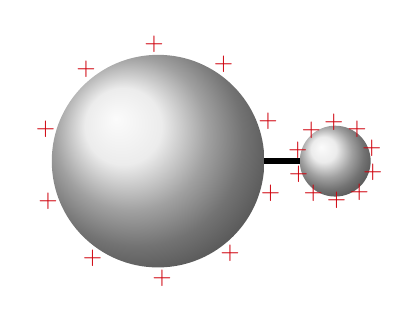
\begin{tikzpicture}[scale=0.45]

  \shade[ball color = gray!20, opacity = 1] (0,0) circle (3cm);
  \shade[ball color = gray!20, opacity = 1] (5,0) circle (1cm);  
  \draw[line width=2pt,black] (3,0)--(4,0) ;
  
  \foreach \i [evaluate={\ang=20+\i*360/10;}] in {1,...,10}{
    \node[myred,scale=0.9] at (\ang:1.1*3) {\textbf{$+$}};
   }
  \begin{scope}[xshift=5cm]  
  \foreach \i [evaluate={\ang=20+\i*360/10;}] in {1,...,10}{
    \node[myred,scale=0.9] at (\ang:1.1) {\textbf{$+$}};
   } 
  \end{scope}
    
\end{tikzpicture}
\captionof*{figure}{\textit{Two connected charged conducting spheres.}}
\end{center}
\only<2>{
\vspace{-0.5cm}
\begin{exampleblock}{Electric field}
The potential is the same on each sphere:
\begin{align*}
V=E_1R_1=E_2R_2
\end{align*}
The \textbf{electric field is strongest where radius of curvature is smallest}.
\end{exampleblock}
}
}


%%%%%%%%%%%%%%%%%%%%%%%%%%%%%%
\subsection{The lightnening rod}
\label{subsec:thelightningrod}
\twocolframesf{The lightening rod}
{

\begin{itemize}
  \item In general, charges get concentrated at the sharp part of a conductor (the charge density and electric field are highest where the radius of curvature is smallest)
  \item This means the electric field there can be very high on a sharp point
  \item[$\rightarrow$] Ideally, the strong electric field allows for corona discharge, and charges can leak from the lighting rod into the cloud
  \item[$\rightarrow$] If the electric field gets too strong, then the air breaks down, and you get lightning!
\end{itemize}
So lighting rods do draw lighting, but ideally, they prevent it all together!
}
{
\vspace{-1cm}
\capfig{1}{figures/Potential/chargeblob}{}
\vspace{-1cm}
 \begin{columns} 
 \column{0.7\textwidth}
 \capfig{1}{figures/Potential/lightningrod}{}
 \column{0.3\textwidth}
 \capfig{1}{figures/Potential/lightning}{}
 \end{columns}
}



%%%%%%%%%%%%%%%%%%%%%%%%%%%%%%
\subsection{Measuring the Van de Graaf terminal voltage}
\label{subsec:measuringthevandergraadterminalvoltage}
\twocolframesf{Measuring the Van der Graaf terminal voltage}
{
\begin{itemize}
  \item We can assume that the electric field is roughly constant between the two spheres (like parallel plates):
  \begin{align*}
  \Delta V = Ed
  \end{align*}
  \item For breakdown in air, $E=\SI{3e6}{V/m}$.
  \item Can measure $d$ on the Van der Graaf to determine its voltage!
\end{itemize}
}
{
\centering
 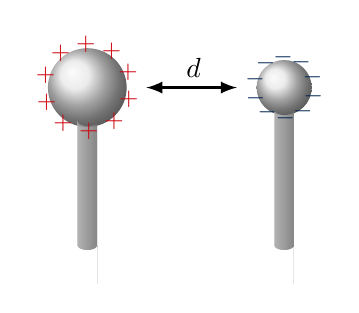
\begin{tikzpicture}[scale=0.5]
  \def\Rout{1.0} 
  %The two balls:
  \shade[ball color = gray!20, opacity = 1] (0,0) circle (1cm);
  \shade[ball color = gray!20, opacity = 1] (5,0) circle (0.7cm);  
  %The arrow with the label on top:
  \draw[line width=1pt,black, latex-latex] (1.5,0)--(3.8,0) ;
  \node at (2.7,0.5) {$d$};
  %The side of a cylinder:
  \fill[left color=gray!20!,right color=gray!80!,shading=axis,opacity=0.6] (0.25,-5) -- (0.25,-0.85) arc (360:180:0.25cm and 0.125cm) -- (-0.25,-4) arc (180:360:0.25cm and 0.125cm);
  
  %The + charges
  \foreach \i [evaluate={\ang=20+\i*360/10;}] in {1,...,10}{
    \node[myred,scale=0.9] at (\ang:1.1) {\textbf{$+$}};
   }
  %Shift scop to the second ball to add its cylinder and - charges
  \begin{scope}[xshift=5cm]  
  \fill[left color=gray!20!,right color=gray!80!,shading=axis,opacity=0.6] (0.25,-5) -- (0.25,-0.57) arc (360:180:0.25cm and 0.125cm) -- (-0.25,-4) arc (180:360:0.25cm and 0.125cm);
  \foreach \i [evaluate={\ang=20+\i*360/10;}] in {1,...,10}{
    \node[myblue,scale=0.9] at (\ang:1.1*0.7) {\textbf{$-$}};
   } 
  \end{scope}
\end{tikzpicture}
\captionof*{figure}{\textit{The two terminals of a Van der Graaf generator, separated by a distance $d$.}}
 
}

%%%%%%%%%%%%%%%%%%%%%%%%%%%%%%



%%%%%%%%%%%%%%%%%%%%%%%%%%%%%%



%%%%%%%%%%%%%%%%%%%%%%%%%%%%%%
\def\dipole at (#1,#2,#3){
\tikzmath{
 \dipoleL=0.25;
 \dipoleR=0.1;
}

\begin{scope}[shift={(#1,#2)}, rotate=#3]
  \fill[color=myblue!40,draw=black] (-\dipoleR,-\dipoleL/2) -- (-\dipoleR, \dipoleL/2) arc(180:0:\dipoleR) -- (\dipoleR, -\dipoleL/2) arc(0:-180:\dipoleR) --cycle;
  \node[color=white] at (0,+\dipoleL/2){\tiny ${+}$};
  \node[color=white] at (0,-\dipoleL/2){\tiny ${-}$};
\end{scope}
}

\subsection{Capacitors}
\label{subsec:capacitors}
\twocolframesf{Capacitors}
{
\begin{itemize}
\item Capacitors are a way to store charges.
\item Two electrodes, always equal and opposite charge, $+Q$ and $-Q$, held at a potential difference, $\Delta V$ (imagine parallel plates).
\item Geometry determines how much charge you can store on a capacitor for a given voltage, the ``capacitance'', $C$:
\begin{align*}
Q=C\Delta V
\end{align*}
\item The capacitor stores electric potential energy:
\begin{align*}
U = \frac{1}{2}\frac{Q^2}{C^2}=\frac{1}{2}C\Delta V^2 = \frac{1}{2}Q\Delta V
\end{align*}
\end{itemize}
}
{
\only<1>{
\begin{center}
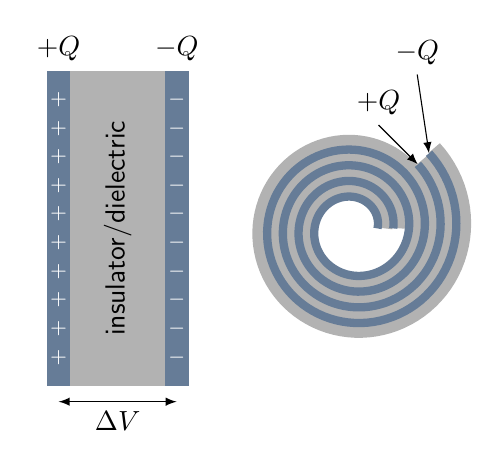
\begin{tikzpicture}
\tikzmath{
\L=1.5;
\h=4;
\platew=0.3;
}
\scalebox{1}{

\fill[color=myblue!60] (-\L/2-\platew/2,-\h/2) rectangle +(\platew,\h);
\fill[color=myblue!60] (\L/2-\platew/2,-\h/2) rectangle +(\platew,\h);
\fill[color=black!30] (-\L/2+\platew/2,-\h/2) rectangle (\L/2-\platew/2,\h/2);
 %charges
 \foreach \i in{1,...,10}{
   \node[color=white] at (-\L/2,-\h/2+\i*\h/11) {\scriptsize $+$};
   \node[color=white] at (\L/2,-\h/2+\i*\h/11) {\scriptsize $-$};
 }
 \node[above] at (-\L/2,\h/2){$+Q$};
 \node[above] at (\L/2,\h/2){$-Q$};
 \node[rotate=90] at (0,0){insulator/dielectric};
\draw[latex-latex] (-\L/2,-\h/2-0.2) -- +(\L,0) node[midway,below]{$\Delta V$};
\begin{scope}[shift={(2*\L,0)}]

\draw[color=black!30, line width=5] plot[variable=\x,domain=0:765,samples=200] (\x:{0.4+0.4*\x/360});%dielectric
\draw[color=black!30, line width=5] plot[variable=\x,domain=0:765,samples=200] (\x:{0.6+0.4*\x/360});%dielectric
\draw[color=myblue!60, line width=3] plot[variable=\x,domain=0:765,samples=200] (\x:{0.3+0.4*\x/360});%+Q
\draw[color=myblue!60, line width=3] plot[variable=\x,domain=0:765,samples=200] (\x:{0.5+0.4*\x/360});%-Q

\draw[latex-] (45:1.15) -- +(-0.5,0.5) node[above]{$+Q$};
\draw[latex-] (45:1.35) -- +(-0.15,1) node[above]{$-Q$};
\end{scope} 

}
\end{tikzpicture}
\captionof*{figure}{\textit{Different capacitor geometries.}}
\end{center}
}
%Dielectric with and without field
\only<2>{
\begin{center}

\begin{tikzpicture}
\tikzmath{
\L=2.5;
\h=1.5;
\platew=0.2;
}
\scalebox{1}{
 %plates and dielectric
 \fill[color=myblue!60] (-\L/2,-\h/2-\platew/2) rectangle +(\L,\platew);
 \fill[color=myblue!60] (-\L/2,\h/2-\platew/2) rectangle +(\L,\platew);
 \fill[color=black!30] (-\L/2,-\h/2+\platew/2) rectangle (\L/2,\h/2-\platew/2);
 %dipoles
 \foreach \i in{1,...,4}{
   \dipole at (-\L/2+\i*\L/5,-\h/4,360*random()) ;
   \dipole at (-\L/2+\i*\L/5,\h/4,360*random()) ;
 }
 
\begin{scope}[shift={(1.25*\L,0)}]
 \fill[color=myblue!60] (-\L/2,-\h/2-\platew/2) rectangle +(\L,\platew);
 \fill[color=myblue!60] (-\L/2,\h/2-\platew/2) rectangle +(\L,\platew);
 \fill[color=black!30] (-\L/2,-\h/2+\platew/2) rectangle (\L/2,\h/2-\platew/2);
  %dipoles
 \foreach \i in{1,...,4}{
   \dipole at (-\L/2+\i*\L/5,-\h/4,0) ;
   \dipole at (-\L/2+\i*\L/5,\h/4,0) ;
 }

 %charges on plates
 \foreach \i in{1,...,6}{
   \node[color=white] at (-\L/2+\i*\L/7,-\h/2) {\scriptsize $+$};
   \node[color=white] at (-\L/2+\i*\L/7,\h/2) {\scriptsize $-$};  
 }

\end{scope}
}
\end{tikzpicture}
\captionof*{figure}{\textit{Dielectric materials contain little dipoles; by re-orienting them, we can store energy.}}
\end{center}
\begin{block}{Dielectrics}
The capacitance also depends on the properties of the material between the plates. More energy is stored by using
a dielectric material (one that can polarize). The dielectric lowers the field between the plates, allowing for more
charges at a given voltage. 
\end{block}
}

}
%%%%%%%%%%%%%%%%%%%%%%%%%%%%%%


%%%%%%%%%%%%%%%%%%%%%%%%%%%%%%%%%



%%%%%%%%%%%%%%%%%%%%%%%%%%%%%%%%



\end{document}
